\section{Benutzeroberfläche der Anwendung}
In diesem Kapitel wird die Benutzeroberfläche der Anwendung beschrieben. Die Anwendung ist dafür ausgelegt den PV-Batterie-Besitzer eine schnelle und einfache Antwort auf die Frage zu geben, ob die Teilnahme an einem virtuellen Kraftwerk auf Basis der SonnenFlat sinnvoll ist. \medskip

Die Oberfläche besteht aus den zwei Tabs "Basis Einstellungen" und "Erweitert". Auf der zuerst sichtbaren Seite "Basis Einstellungen" werden die grundlegenden Systemparameter bestimmt. Die gewünschten Werte für die installierte PV-Leistung, die Batteriekapazität und den Stromverbrauch pro Jahr stellt man, wie schon in den Übungen, über drei Schieberegler ein. Zwei farbige Tortendiagramme bilden anteilig die Solarstromnutzung und die Zusammensetzung der Stromversorgung des Haushalts ab. Der jeweilige Eigenverbrauchsanteil und Autarkiegrad wird zusätzlich als Dezimalzahl dargestellt. Zusätzlich besteht die Möglichkeit mit einem Schalter die Kennzahlen und Diagramme mit und ohne Regelleistungserbringung zu vergleichen. \\
\begin{figure}[H]
	\begin{center}
		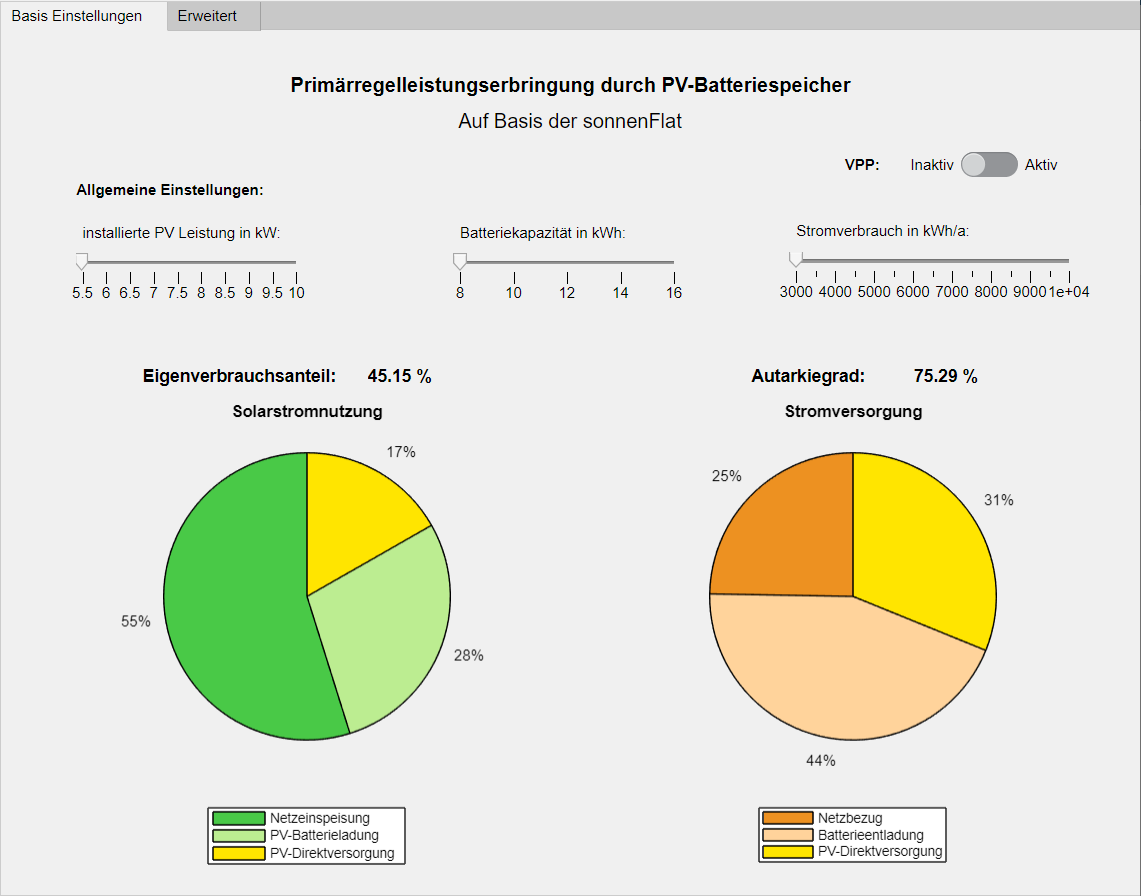
\includegraphics[width=\textwidth]{Bilder/N_ScreenshotApp1.png}
		\caption{Startseite der Anwendung}
		\label{fig:app1}
	\end{center}
\end{figure}

Der Schwerpunkt des zweiten Tabs liegt darin zu zeigen, ob sich das System finanziell für den Verbraucher rechnet. Zuerst wird der bisherige Stromtarif über die Regler für die Fixkosten und variablen Kosten eingestellt. Als nächstes kann die EEG-Vergütung, die man erhält, über ein Dropdown-Menü ausgewählt werden. Mithilfe der angegebenen Parameter entsteht Balkendiagramm, das die berechneten Kosten und Einnahmen mit und ohne virtuelles Kraftwerk übersichtlich gegenüberstellt. Die Kosten sind orange, bzw. negativ aufgetragen und die Einnahmen und der EEG-Bonus ist grün, bzw. positiv aufgetragen.  Darunter abgebildet sind außerdem die sich ergebenden Jahresbilanzen, sowie die Differenz dieser. Ist die Differenz positiv, d. h. kann mit dem virtuellen Kraftwerk Geld gespart oder mehr verdient werden, leuchtet das Lämpchen grün. In diesem Fall ist Einsatz des Speichers als Teil des virtuellen Kraftwerks zu empfehlen. Leuchtet das Lämpchen rot, ist davon abzuraten.
\begin{figure}[H]
	\begin{center}
		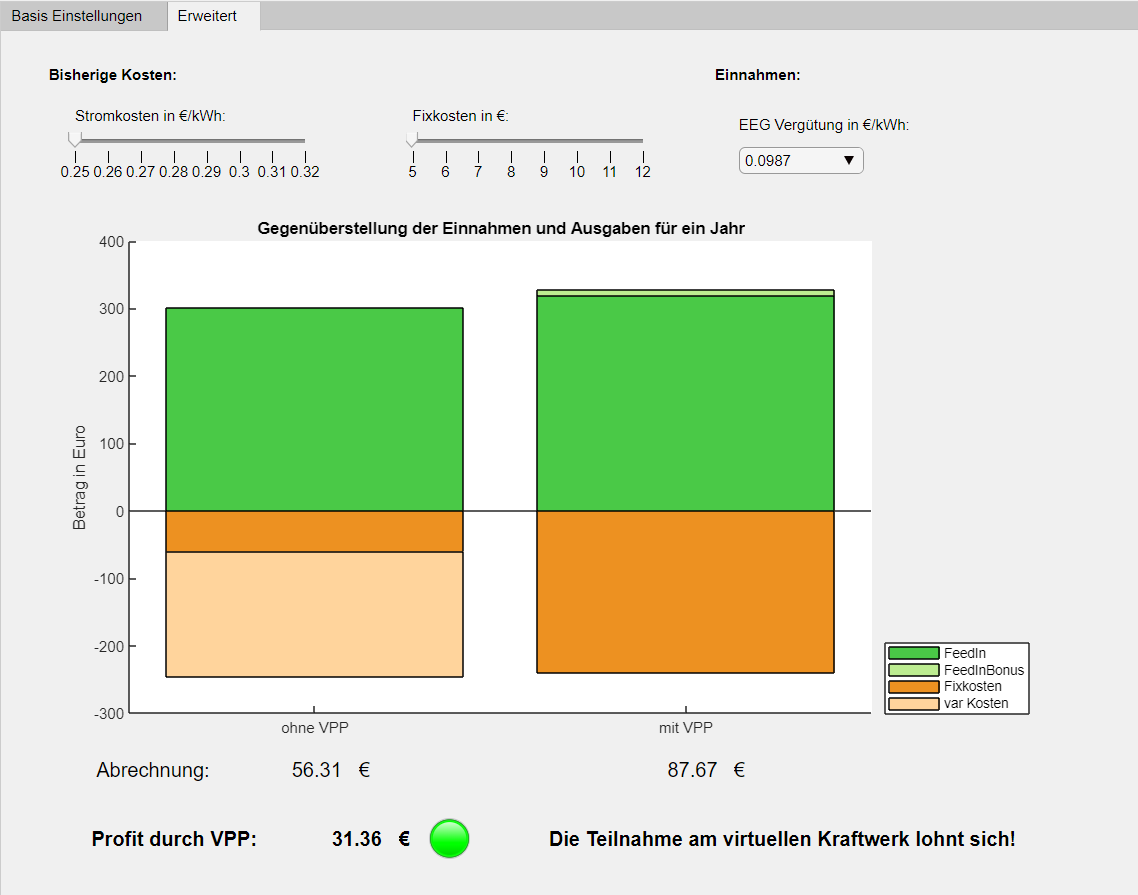
\includegraphics[width=\textwidth]{Bilder/N_ScreenshotApp2.png}
		\caption{Zweite Seite der Anwendung}
		\label{fig:app2}
	\end{center}
\end{figure}



\section{Ergebnisauswertung}

In den nachfolgenden Abschnitten werden die wichtigsten Ergebnisse der Simulation dargestellt und untersucht. Außerdem werden die relevanten Parameter einer Sensibilitätsanalyse unterzogen, um ihren Einfluss auf die Resultate zu quantifizieren.\medskip

\subsection{Ergebnisdarstellung}
Zunächst werden die entstandenen Extrempunkte betrachtet. Da das Ziel des Projekts primär die wirtschaftliche Beurteilung der Regelleistungserbringung durch PV-Batteriespeicher ist, werden die Fälle untersucht, in denen der direkte und indirekte finanzielle Verlust und Gewinn maximal sind. \\
Um diese Bedingungen zu definieren werden folgende Annahmen getroffen. Es ist davon auszugehen, dass bei aktivem VPP mehr Energie durch die PV-Anlage in das Netz eingespeist wird, da die Batterie aufgrund der geltenden SoC-Grenzen eine geringere Speicherkapazität bietet. Deswegen unterliegt der höchstmögliche Gewinn durch das VPP der Bedingung, dass die EEG Vergütung maximal ist. Umgekehrt ist der größte Verlust durch das VPP bei minimaler EEG Vergütung zu erwarten. Die Fixkosten und variablen Kosten, die nur die Bilanz ohne VPP beeinflussen, haben hingegen eine genau gegenteilige Wirkung. Je höher sie sind, desto günstiger ist es für den Wechsel zur SonnenFlat. \\
Die einzelnen Einnahme- und Kostenpunkte für die Extrempunkte sind in \ref{fig:Bilanz_minmax} aufgetragen. Das obere Balkendiagramm zeigt den günstigsten Fall. Konkret wird erreicht sich Maximum der Bilanzdifferenz bei 
\begin{itemize}
\itemsep-0.5em
	\item Einem Hausverbrauch von 10000{\kwh}
	\item Einer Kapazität der Batterie von 14{\kwh}
	\item Einer Größe der Photovoltaikanlage von 9.5{\kwp}
	\item Einer EEG-Vergütung für die Stromeinspeisung von 12.75{\ctkwh}
	\item Einem Grundpreis des Vergleichstromtarifs von 12{\Eurkwh}
	\item Einem Arbeitspreis des Vergleichstromtarifs von 32{\ctkwh}
\end{itemize}
erreicht. Die Einnahmen durch die Wirkung des VPPs belaufen sich auf maximal 849.02 Euro\\•
Die Zusammensetzung des Minimums der Bilanzdifferenz wird im unteren Diagramm abgebildet und befindet sich bei
\begin{itemize}
\itemsep-0.5em
	\item Einem Hausverbrauch von \SI{10000}{\kwh}
	\item Einer Kapazität der Batterie von \SI{16}{\kwh}
	\item Einer Größe der Photovoltaikanlage von \SI{7}{\kwp}
	\item Einer EEG-Vergütung für die Stromeinspeisung von \SI{9.87}{\ctkwh}
	\item Einem Grundpreis des Vergleichstromtarifs von \SI{5}{\Eurkwh}
	\item Einem Arbeitspreis des Vergleichstromtarifs von \SI{25}{\ctkwh}
\end{itemize}
Der maximale Verlust durch das VPP beträgt -321,60 Euro.
\begin{figure}[H]
	\begin{center}
		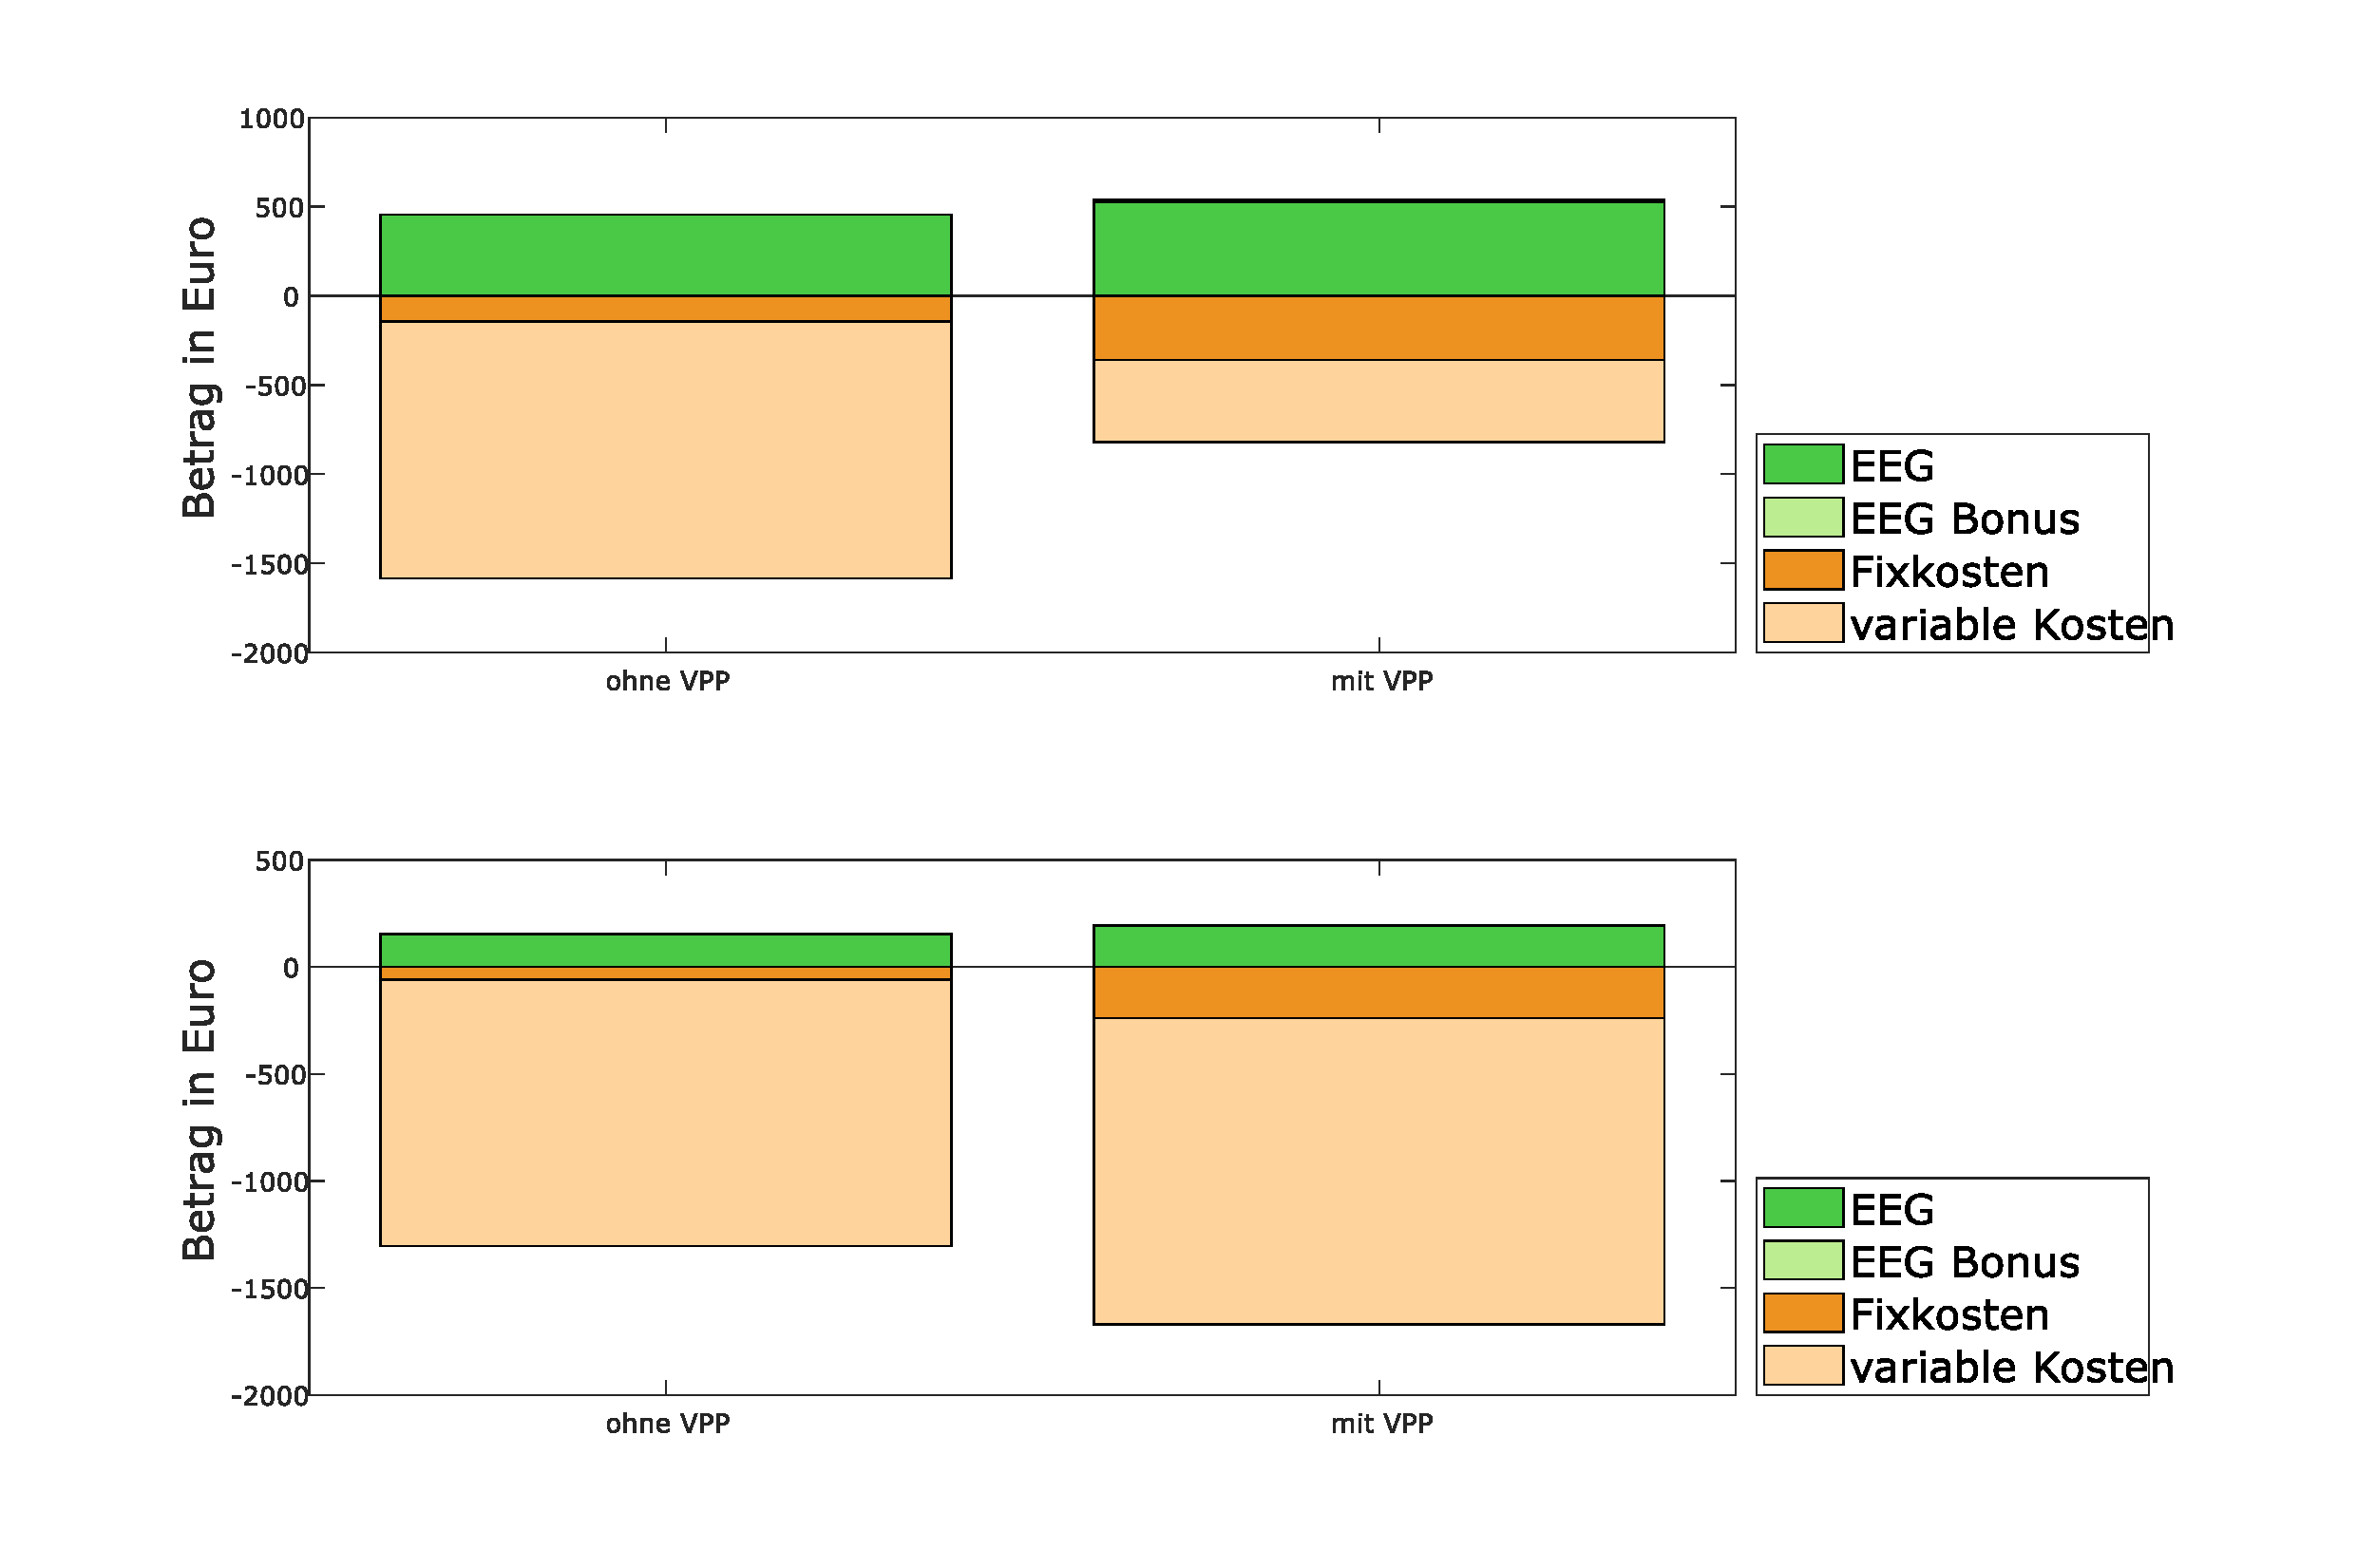
\includegraphics[width=\textwidth]{Bilder/Gegenueberstellung_Bilanz.pdf}
		\caption{Gegenüberstellung der Einnahmen und Kosten für den Verbraucher in zwei Fällen jeweils mit und ohne Regelleistungsbereitstellung für ein Jahr}
		\label{fig:Bilanz_minmax}
	\end{center}
\end{figure}

Ein Effekt, der langfristig zu finanziellem Verlust führen kann, ist die Zyklenbeanspruchung des Batteriesystems. Nach der Betrachtung des SoC ist eine höhere Auslastung der Batterie zu erwarten. Eine besonders hohe Zyklenzahl ist zu erwarten bei einer hohen installierten PV-Leistung, niedriger Batteriekapazität und hoher Last. \\
Betrachtet man nun die Simulationsergebnisse bestätigt sich dieser Verdacht.ist kaum ein Unterschied zu erkennen. Allerdings liegt die Anzahl der Zyklen mit VPP nicht übermäßig über der ohne, das Zyklenmaximum ohne VPP ist mit 296 sogar um 15 Ladegänge höher. Und auch das Minimum liegt mit 95 nur 17 niedriger als mit VPP. Nur mit dieser geringen Anzahl an Werten fällt es schwer eine aussagekräftige Wertung über den Einfluss von Regelleistungsbereitstellung abzugeben, wobei sie trotz alledem vermuten lassen, dass er nicht erheblich ist. Hinzu kommt, dass das SonnenBatterie System auch bei einer deutlich höheren Zyklenzahl noch garantiefähig ist, da diese erst nach 10.000 Zyklen bzw. 10 Jahren Gebrauch verfällt \cite{sonnenBat18}.
% Notizen: Hier noch Plot mit Zyklenzahl einbinden!

\subsection{Sensibilitätsanalyse}
% Einfluss der PV Leistung
% Einfluss der Batteriekapazität
% Einfluss der Last
% Einfluss der variablen Kosten
% Einfluss der EEG Umlage


